%
% teil1.tex -- Beispiel-File für das Paper
%
% (c) 2020 Prof Dr Andreas Müller, Hochschule Rapperswil
%
\section{Problemstellung}
\rhead{Problemstellung}
Dank der breiten Anwendung der Matrizenmultiplikation ist eine effiziente L\"osung dieser Operation von grosser Bedeutung.
Das Ziel dieses Papers ist, verschiedenen Algorithmen der Matrizenmultiplikation vorzustellen.
Gezielt werden auf Algorithmen, welche das Problem schneller als der Standard Algorithmus L\"osen eingegangen.

\subsection{Big $\mathcal{O}$ Notation}
Die Big $\mathcal{O}$ Notation beschreibt die Laufzeitkomplexit\"at eines Algorithmus \cite{multiplikation:bigo}.
$f(x) \in \mathcal{O}(g(x))$ besagt, dass die Funktion $f$ nicht wesentlich schneller w\"achst als $g$ wenn $x \rightarrow \infty$.
Vereinfacht werden f\"ur Algorithmen die folgende Notation verwendet:
\begin{itemize}
	\item $f \in \mathcal{O}(1) \rightarrow f$ ist beschr\"ankt
	\item $f \in \mathcal{O}(n) \rightarrow f$ w\"achst linear
	\item $f \in \mathcal{O}\left (n^2 \right ) \rightarrow f$ w\"achst quadratisch
	\item $f \in \mathcal{O}(\log n) \rightarrow f$ w\"achst logarithmisch
	\item $f \in \mathcal{O}(n \log n) \rightarrow f$ hat super-lineares Wachstum
	\item $f \in \mathcal{O}\left (e^n \right ) \rightarrow f$ w\"achst exponentiell
	\item usw.
\end{itemize}

In der Abbildung \ref{multiplikation:fig:bigo} k\"onnen die verschiedenen Laufzeiten miteinander verglichen werden. 

\begin{figure}
	\center
	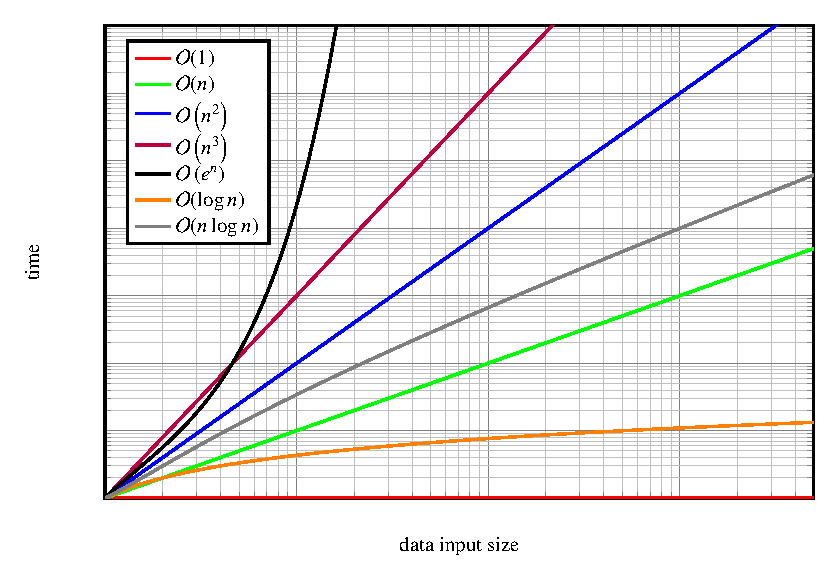
\includegraphics[]{papers/multiplikation/images/bigo}
	\caption{Verschiedene Laufzeiten}
	\label{multiplikation:fig:bigo}
\end{figure}

\subsubsection{Beispiel Algorithmen}

Folgend einige Beispiele von Algorithmen welche zu einer bestimmten Zeitkomplexit\"atsklassen geh\"oren.
\paragraph{Beschr\"ankter Algorithmus}

Ein Beispiel eines Beschr\"ankter Verhalten $\mathcal{O}(1)$, kann im Algorithmus \ref{multiplikation:alg:b1} entnommen werden. Da $a$ und $b$ Skalare sind, hat keine Gr\"osse $n$ einen einfluss auf die Laufzeit.

\begin{algorithm}\caption{}
	\label{multiplikation:alg:b1}
	\setlength{\lineskip}{7pt}
	\begin{algorithmic}
		\Function{B1}{$a, b$}
		\State \textbf{return} $a+b$
		\EndFunction
	\end{algorithmic}
\end{algorithm}

Konstanten werden nicht beachtet, der Algorithmus \ref{multiplikation:alg:b2} f\"uhrt ebenso zu  $\mathcal{O}(1)$ und nicht zu $\mathcal{O}(2)$.

\begin{algorithm}\caption{}
	\label{multiplikation:alg:b2}
	\setlength{\lineskip}{7pt}
	\begin{algorithmic}
		\Function{B2}{$a, b$}
		\State $ x \gets a+b $
		\State $ y \gets a \cdot b $
		\State \textbf{return} $x+y$
		\EndFunction
	\end{algorithmic}
\end{algorithm}

\paragraph{Linearer Algorithmus}

Folgender Algorithmus \ref{multiplikation:alg:l1} hat ein lineares Verhalten.
Die \texttt{for}-Schleife wird $n$-mal durchgef\"hrt und f\"uhrt deshalb zu $\mathcal{O}(n)$.

\begin{algorithm}\caption{}
	\setlength{\lineskip}{7pt}
	\begin{algorithmic}
		\label{multiplikation:alg:l1}
		\Function{L}{$\mathbf{a}, \mathbf{b}$,n}
		\State $ sum \gets 0$
		\For{$i = 0,1,2 \dots,n$}
		\State $ sum \gets sum + A[i] \cdot B[i] $
		\EndFor
		
		\State \textbf{return} $sum$
		
		\EndFunction
	\end{algorithmic}
\end{algorithm}

\paragraph{Quadratischer Algorithmus}

Folgender Algorithmus \ref{multiplikation:alg:q1} hat ein quadratisches Verhalten.
Die beiden \texttt{for}-Schleifen werden jeweils $n$-mal durchgef\"hrt und f\"uhrt deshalb zu $\mathcal{O}\left(n^2\right)$.


\begin{algorithm}[H]\caption{}
	\label{multiplikation:alg:q1}
	\setlength{\lineskip}{7pt}
	\begin{algorithmic}
		\Function{Q}{$\mathbf{A}, \mathbf{B}$,n}
		\State $ sum \gets 0$
		\For{$i = 0,1,2 \dots,n$}
		\For{$j = 0,1,2 \dots,n$}
		\State $ sum \gets sum + A[i] \cdot B[j] $
		\EndFor
		\EndFor
		\State \textbf{return} $sum$
		\EndFunction
	\end{algorithmic}
\end{algorithm}


